\documentclass{jknotes}
\usepackage{joshkirklin,pgfplots}

\tikzset{
    partial ellipse/.style args={#1:#2:#3}{
        insert path={+ (#1:#3) arc (#1:#2:#3)}
    }
}

\newcommand{\dunder}[1]{\underline{\underline{#1}}}
\renewcommand{\trace}[1]{\text{tr}\left(#1\right)}
\newcommand{\srate}{\dot{\gamma}}
\usetikzlibrary{intersections, pgfplots.fillbetween}

\begin{document}

\institution{Cambridge Part III Maths}
\title{Non-Newtonian Fluid Mechanics}
\lecturer{Eric Lauga}
\notetaker{Charles Powell}
\date{Michaelmas 2020}

\maketitle
\suggestionsspiel
\tableofcontents

\section{Introduction to Non-Newtonian Fluids}
\lecture{08/10/20}
Newtonian fluids are typically characterised by 2 material properties:
viscosity and density. We may also refer to Newtonian fluids as `simple
fluids'.


Non-Newtonian fluids may have many other material properties, for example
intrinisic time, length and stress scales, and an intrinsic orientation. They
often exhibit a mix of fluid and solid behaviour. We may also refer to
non-Newtonian fluids as `complex fluids'.


There are many examples of complex fluids readily apparent in our everyday
lives, for example sand (wet or dry) and mud; lava and glass, both of which
experience phase changes; ketchup; foam; paint; emulsions such as milk; liquid
crystals used in screens; blood on very small scales.


The goal of this course is to cover three main areas.
\begin{itemize}
	\item Phenomenology of non-Newtonian fluids -- how do they behave?
	\item Mathematical modelling -- how do we quantify the behaviour?
	\item Predictions (and limits) of models
\end{itemize}

\section{Summary of Newtonian Fluid Mechanics}
\subsection{Continuum approximation}
We describe fluids in terms of two main fields: \emph{density} $\rho(\bm{x},t)$  and
\emph{velocity} $\bm{u}(\bm{x},t)$. We use the continuum approximation whereby the
fluid is assumed to be a continuum rather than made up of discrete fluid
particles. Under this assumption, the macroscopic properties of density and
velocity are well-defined as `averages' of infinitesimal volume elements. 

The velocity field is \emph{Eulerian}, meaning it is measured at a specific
point in space and time, as opposed to following a material element
(Lagrangian).

\subsection{Conservation of mass}

Conservation of mass can be expressed in the classical form of a conservation
equation as:
\begin{equation}
	\frac{\partial \rho}{\partial t} + \nabla \cdot \left[ \rho \bm{u} \right]
	= 0
\end{equation}

Expanding the flux term, this may be expressed in a form which relates the
rate of change of density of a fluid element with the divergence of the
flow:
\begin{equation}
	\frac{\diffD{\rho}}{\diffD{t}} = -\rho \nabla \cdot \bm{u}
\end{equation}

In this course we will assume that all fluids are incompressible, which is
expressed mathematically as:
\begin{equation}
	\frac{\diffD{\rho}}{\diffD{t}} = 0 \iff \nabla \cdot \bm{u} = 0
\end{equation}

\subsection{Mechanical equilibrium}
Newton's second law, i.e. conservation of momentum is expressed for a fluid
using the \emph{Cauchy momentum equation}:
\begin{equation}
	\rho \frac{\diffD{\bm{u}}}{\diffD{t}} = \rho \left[ \frac{\partial
	\bm{u}}{\partial t} + \bm{u} \cdot \nabla \bm{u}\right] = \nabla \cdot
	\sigma + \bm{F}
\end{equation}

where $\nabla \cdot \sigma$ are the surface forces acting on the fluid and
$\bm{F}$ are body forces which we will assume to be negligible unless
otherwise stated.
 
The Cauchy momentum equation is valid for all continuum fluids. To close the
equation, we require an expression for $\sigma$.

\begin{defn}
The \emph{stress tensor} $\sigma$ is a symmetric second-rank tensor.
\begin{center}
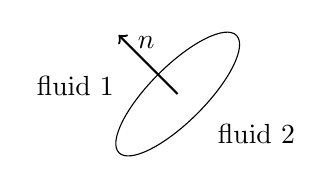
\begin{tikzpicture}
	\draw[rotate=45] (0,0) ellipse (30pt and 10pt);
	\draw[->, thick] (0,0) -- (-.75,.75);
	\node at (-0.4,0.65) {$\bm{n}$};
	\node at (-1.3,0.1) {fluid 1};
	\node at (1,-0.5) {fluid 2};
\end{tikzpicture}
\end{center}
Physically, $\sigma_{ij}n_j$ is the $i\textsuperscript{th}$ component of the force per
unit area from the motion of fluid 1 on fluid 2, where $\bm{n}$ is the
surface normal pointing into fluid 1.
\end{defn}

\subsection{Constitutive modelling}
The stress tensor is specified in terms of the deformation via \emph{constitutive
modelling}.

\begin{eg}{Newton's experiment\\}
Consider two parallel plates of area $A$ separated a distance $h$ by a fluid.
We consider the force $F$ required on the top plate to induce motion at speed
$U$. Note that there is no force perpendicular to the plates if the fluid is
Newtonian. This is not necessarily true for complex fluids.
\begin{center}
	\begin{tikzpicture}
		\begin{axis}[scatter/classes={a={mark=x,draw=black}},yticklabels={,,},xticklabels={,,},xlabel={$U/h$},ylabel={$F/A$},xmin=0,xmax=5,ymin=0,ymax=5]
		\addplot[scatter,only marks, scatter src = explicit symbolic]
		table[meta = label] {
			x y label 
			0.98 1 a
			1.5 1.48 a
			2 2.03 a
			2.43 2.39 a
			3.03 3.01 a
			3.45 3.55 a
			4.01 4 a
		};
		\addplot[no marks, black, dashed]{x};
	\end{axis}
	\end{tikzpicture}
\end{center}

From experiment, we find $\sigma = F/A \propto U/h$. Note that $U/h$ has
dimensions of time$^{-1}$. We define the \emph{shear rate} $\dot{\gamma} =
U/h$ and the \emph{viscosity} $\eta$ via $\sigma = \eta \dot{\gamma}$.
Viscosity is a constant material property, for example in water $\eta =
10^{-3}\, \text{Pa}\cdot\text{s}$.

\end{eg}

We can now generalise for all Newtonian flows. We start by separating out an
isotropic component of the shear tensor:
\begin{equation}
	\sigma_{ij} = -p \delta_{ij} + \tau_{ij}
\end{equation}
where $p$ is the \emph{dynamic pressure} and $\tau$ is the \emph{deviatoric
stress}. The deviatoric stress may be a function of $u_i, \frac{\partial u_i}{\partial
x_j}, \dots$; local or non-local in time or space; or a function of other
material properties and parameters. For Newtonian fluids, we make five
assumptions.

\begin{enumerate}
	\item Galilean invariance: the deviatoric stress cannot depend on $u_i$
	\item Instaneous response: there is no dependence on the history of
		deformation
	\item Locality: no dependence on second or higher spatial derivatives
	\item Linearity: $\tau_{ij}$ is linearly related to $\frac{\partial
		u_m}{\partial x_n}$
	\item Isotropy: the relationship is independent of reference frame, i.e.
		isotropic
\end{enumerate}

We can satisfy 1, 2, 3, and 4 by writing
\begin{equation}
	\tau_{ij} = A_{ijkl}\frac{\partial u_k}{\partial x_l}
\end{equation}
where $A_{ijkl}$ is a fourth rank tensor. Using the form of the most general
isotropic fourth rank tensor we may enforce isotropy.
\begin{equation}
	A_{ijkl} = A \delta_{ij} \delta_{kl} + B \delta_{ik}\delta_{jl} + C
	\delta_{il}\delta_{jk}
\end{equation}

Since $\sigma$ is symmetric, $\tau$ is symmetric, therefore $A_{ijkl} =
A_{jikl}$. This requires $B = C \equiv \eta$. Thus
\begin{equation}
	\begin{aligned}
		\tau_{ij} &= A\delta_{ij} \frac{\partial u_k}{\partial x_k} + \eta
		\left( \frac{\partial u_i}{\partial x_j} + \frac{\partial
		u_j}{\partial x_i} \right) \\
		&= \eta \left( \frac{\partial u_i}{\partial x_j} + \frac{\partial
		u_j}{\partial x_i} \right) \\
		&= 2 \eta e_{ij}
	\end{aligned}
\end{equation}

since $\frac{\partial u_k}{\partial x_k} = \nabla \cdot \bm{u} = 0$. Note
$e = \frac{1}{2}\left(\nabla \bm{u} + (\nabla \bm{u})^T\right)$ is the
\emph{rate of strain} tensor. This is the \emph{Newtonian constitutive
	relationship}. 
	
\begin{defn}
	To exclude the factors of $2$ we define the \emph{shear rate}
	$\dot{\gamma}_{ij} = 2 e_{ij}$ so that $\tau_{ij} = \eta
	\dot{\gamma}_{ij}$.
\end{defn}

Combining the Cauchy momentum equation and Newtonian constitutive relationship
yields the \emph{Navier-Stokes equations}
\begin{equation}
	\rho \frac{\diffD{\bm{u}}}{\diffD{t}} = - \nabla p + \eta \nabla^2 \bm{u}
\end{equation}

Consider a general body with intrinsic length scale $L$, velocity length scale
$U$ and unsteady motion frequency scale $\omega$. Two dimensionless numbers
are used to quantify the importance of inertia:
\begin{equation}
	\text{Re} = \frac{\rho U L}{\eta}, \hspace{2em} \text{Re}_\omega =
	\frac{\rho \omega L^2}{\eta}
\end{equation}

We will assume throughout this course that $\text{Re} \ll 1$ and
$\text{Re}_\omega \ll 1$ unless otherwise stated. In this no-inertia limit,
the Navier-Stokes equations simplify to the \emph{Stokes equations}. For a
general fluid these are:
\begin{equation}
	\nabla \cdot \sigma = 0
\end{equation}

Using the Newtonian constitutive relationship, the Stokes equations are:
\begin{equation}
	\bm{0} = -\nabla p + \eta \nabla^2 \bm{u}
\end{equation}

\begin{eg}{Newton's experiment revisited\\}
	We will apply the above theory to Newton's experiment and show the same
	results are obtained.

	\begin{center}
		\begin{tikzpicture}
			\node at (0,2) {$y = h$};
			\draw (0.6, 2) -- (5, 2);
			\node at (0,0) {$y=0$};
			\draw (0.6, 0) -- (5,0);
			\node at (2.5, 2.5) {$U$};
			\draw[->, thick] (2.15, 2.25) -- (2.85, 2.25);
			\draw[->] (1,0.5) -- (1.6, 0.5) node[midway,below] {$\hat{\bm{x}}$};
			\draw[->] (1,0.5) -- (1, 1.1) node[midway, left] {$\hat{\bm{y}}$};
		\end{tikzpicture}
	\end{center}

	Assume the flow is unidirectional: $\bm{u} = u(y) \hat{\bm{x}}$. The
	Stokes equations become
	\begin{equation}
	\begin{cases}
		\frac{\partial p}{\partial x} = \eta \frac{\partial^2 u}{\partial y^2}
		& = \text{const.}
		\\
		\frac{\partial  p}{\partial y} = 0 & \implies p=p(x)
	\end{cases}
	\end{equation}

	Assuming there is no net pressure drop, $p = p(x) \equiv 0$. Applying the
	boundary conditions we find 
	\begin{equation}
		u(y) = Uy/h \implies \dot{\gamma} = U/h
	\end{equation}
	as before. This is a \emph{shear} or \emph{Couette} flow.
\end{eg}

\lecture{13/10/20}
\section{Phenomenology}

There are four distinguishing properties of non-Newtonian fluids which differ
to Newtonian fluids.

\subsection{Shear-dependent viscosity}
Newtonian fluids have a constant viscosity $\eta$ which is a constant of
proportionality between shear stress $\sigma$ and shear rate $\dot{\gamma}$.
For a complex fluid, $\eta$ is \emph{not} constant. We re-define viscosity as
an implicit function of shear rate.
\begin{defn}
	Viscosity is defined via $\eta \equiv \frac{\sigma}{\dot{\gamma}} =
	\eta(\dot{\gamma})$.
\end{defn}

We can broadly categorise complex fluids into two types: \emph{shear thinning}
and \emph{shear thickening} fluids.

\begin{center}
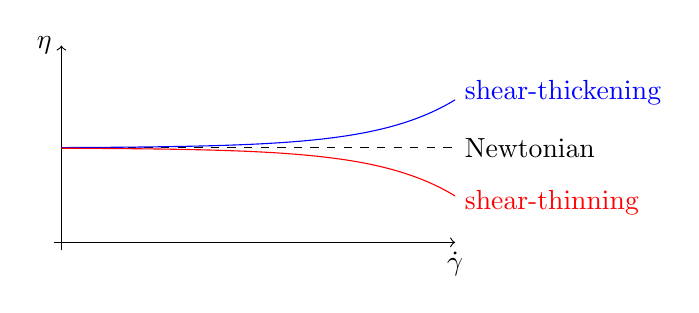
\begin{tikzpicture}
	\draw[->] (-0.1,0) -- (5,0) node[below] {$\dot{\gamma}$};
	\draw[->] (0,-0.1) -- (0,2.5) node[left] {$\eta$};
	\draw[dashed] (0,1.2) -- (5, 1.2) node[right] {Newtonian};
	\draw[smooth,samples=100,domain=0:5,blue] plot(\x, {1.2+0.5*exp(\x-4.8)});
	\draw[smooth,samples=100,domain=0:5,red] plot(\x, {1.2-0.5*exp(\x-4.8)});
	\draw (5, 1.9) node[right,blue] {shear-thickening};
	\draw (5, 0.5) node[right,red] {shear-thinning};
\end{tikzpicture}
\end{center}

Examples of shear-thinning fluids are polymer suspensions; paint; blood. These
complex fluids have $\frac{\partial \eta}{\partial \dot{\gamma}} < 0$.

Examples of shear-thickening fluids are: cornstarch in water; suspesions of
colloidal particles. These complex fluids have $\frac{\partial \eta}{\partial
\dot{\gamma}} > 0$.

\begin{defn}
	The zero-shear rate viscosity is $\eta_0 = \lim_{\dot{\gamma} \to 0}
	\eta$.
\end{defn}

Note that some complex fluids have approximately constant viscosity (Boger
fluids).

\subsection{Fluid memory}
Consider a step-shear flow, that is, Newton's experiment where the top place
impulsively starts motion at $t=0^+$. The response of a Newtonian fluid is on
an inertial timescale $\tau \sim h^2/\nu$ which is almost instantaneous,
whilst a non-Newtonian fluid takes time to respond to adjust to the change in
deformation: the jump occurs over some \emph{relaxation timescale} $\lambda$.

\begin{center}
	\begin{tikzpicture}
		\draw[->] (0,-0.1) -- (0,2.5) node[left] {$\dot{\gamma}$};
		\draw[->] (-0.1,0) -- (5,0) node[below] {$t$};
		\draw (1, -0.1) -- (1, 0.1) node[below] {$t=0$};
		\draw[blue,thick] (0,0) -- (1, 0);
		\draw[blue,thick] (1, 1.2) -- (5, 1.2);
		\draw[blue] (5, 1.4) node[right] {newtonian};
		\draw[red] (5, 1) node[right] {complex};
	\end{tikzpicture}
	\qquad
	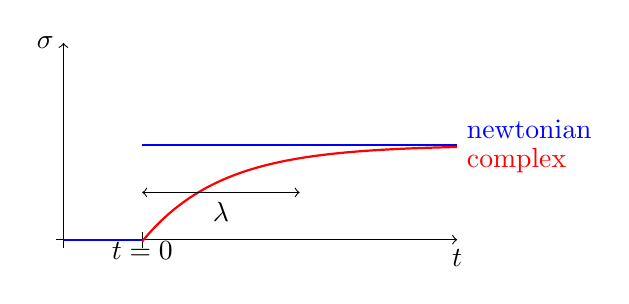
\begin{tikzpicture}
		\draw[->] (0,-0.1) -- (0,2.5) node[left] {$\sigma$};
		\draw[->] (-0.1,0) -- (5,0) node[below] {$t$};
		\draw (1, -0.1) -- (1, 0.1) node[below] {$t=0$};
		\draw[blue,thick] (0,0) -- (1, 0);
		\draw[blue,thick] (1, 1.2) -- (5, 1.2);
		\draw[red, thick, smooth, samples=100, domain=1:5] plot(\x, {1.2 -
		exp(-\x+1.2)});
		\draw[blue] (5, 1.4) node[right] {newtonian};
		\draw[red] (5, 1) node[right] {complex};
		\draw[<->] (1, 0.6) -- (3, 0.6) node[below, midway] {$\lambda$};
	\end{tikzpicture}
\end{center}

The relationship between stress and deformation is \emph{history dependent}.
Impulsively removing the applied shear (i.e. the plate impulsively comes to
rest) results in \emph{stress relaxation} with $\sigma \sim e^{-t/\lambda}$.

\begin{center}
	\begin{tikzpicture}
		\draw[->] (0,-0.1) -- (0,2.5) node[left] {$\dot{\gamma}$};
		\draw[->] (-0.1,0) -- (5,0) node[below] {$t$};
		\draw (2, -0.1) -- (2, 0.1);
		\draw[blue,thick] (0,1.2) -- (2, 1.2);
		\draw[blue,thick] (2, 0) -- (5, 0);
		\draw[blue] (5, 1.4) node[right] {Newtonian};
		\draw[red] (5, 1) node[right] {complex};
	\end{tikzpicture}
	\qquad
	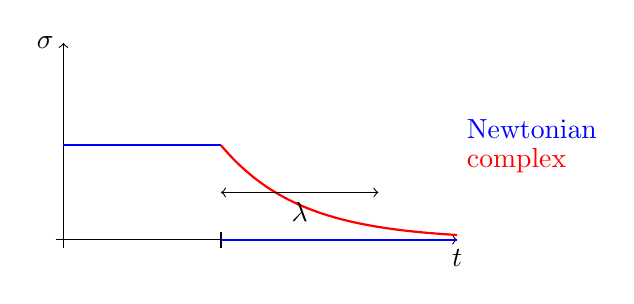
\begin{tikzpicture}
		\draw[->] (0,-0.1) -- (0,2.5) node[left] {$\sigma$};
		\draw[->] (-0.1,0) -- (5,0) node[below] {$t$};
		\draw (2, -0.1) -- (2, 0.1);
		\draw[blue,thick] (0,1.2) -- (2, 1.2);
		\draw[blue,thick] (2, 0) -- (5, 0);
		\draw[red, thick, smooth, samples=100, domain=2:5] plot({\x},
		{1.2*exp(-\x+2)});
		\draw[blue] (5, 1.4) node[right] {Newtonian};
		\draw[red] (5, 1) node[right] {complex};
		\draw[<->] (2, 0.6) -- (4, 0.6) node[below, midway] {$\lambda$};
	\end{tikzpicture}
\end{center}

The reverse is also true. Imposing a stress $\sigma$ and measuring the
deformation $\dot{\gamma}$, complex fluids in general wil have a
history-dependent response. This is called \emph{strain retardation} and
$\lambda'$ is the \emph{retardation timescale}.

\subsection{Normal stress differences}
In Newton's experiment, a Newtonian fluid exerts no normal force $F_N$ on the moving
plate, since linearity and reversibility ($U \to -U$) impies $F_N = -F_N
\equiv 0$. We previously calculated 
\begin{equation}
	\bm{u} = \frac{Uy}{h}\hat{\bm{x}}, \hspace{2em} \dot{\gamma} = \frac{U}{h}
\end{equation}
Thus in the Newtonian case the stress tensor has the form
\begin{equation}
	\sigma = \begin{pmatrix}
		-p_0 & \eta \dot{\gamma} & 0 \\
		\eta \dot{\gamma} & -p_0 & 0 \\
	0 & 0 & -p_0 \end{pmatrix}
\end{equation}
where $p_0$ is the external pressure. Note that the normal stresses are equal
and constant.

In the non-Newtonian case we have
\begin{equation}
	\sigma = \begin{pmatrix}
		\sigma_{xx} & \eta)(\dot{\gamma}) \dot{\gamma} & 0 \\
		\eta(\dot{\gamma}) \dot{\gamma} & \sigma_{yy} & 0 \\
	0 & 0 & \sigma_{zz} \end{pmatrix}
\end{equation}
where in general normal stresses are not equal and not constant. Normal
stresses include the external pressure, so the relevant quantity is the
difference between normal stresses.
\begin{defn}
	The first and second \emph{normal stress differences} are
	\begin{equation}
		N_1 = \sigma_{xx} - \sigma_{yy}, \hspace{2em} N_2 = \sigma_{yy} -
		\sigma_{zz}
	\end{equation}
\end{defn}

Note the following.
\begin{itemize}
	\item For a Newtonian fluid, $N_1 = N_2 = 0$
	\item Polymeric fluids (for example) have $N_1 > 0, N_2 < 0, \left|
		N_2/N_1 \right| \sim 0.1$
	\item $N_1$ and $N_2$ are defined only for steady shear flow
	\item $N_1$ and $N_2$ will, in general, depend on $\dot{\gamma}$
	\item Boger fluids have constant viscosity but they have non-zero $N_1$
		and $N_2$
\end{itemize}

Reversibility implies $N_1$ and $N_2$ have to be \emph{even} functions of
$\dot{\gamma}$. In the limit $\dot{\gamma} \to 0$, i.e. the Newtonian limit,
we should have $N_1 \to 0, N_2 \to 0$. Thus the Taylor expansion of $N_1, N_2$
near $\dot{\gamma} = 0$ is
\begin{equation}
	N_{1,2} = A_{1,2}\dot{\gamma}^2 + B_{1,2}\dot{\gamma}^4 + \dots
\end{equation}

\begin{defn}
	The \emph{normal stress coefficients} are
	\begin{equation}
		\Psi_1 = \frac{N_1}{\dot{\gamma}^2}, \hspace{2em} \Psi_2 =
		\frac{N_2}{\dot{\gamma}^2}
	\end{equation}
\end{defn}

The physical consequence of having normal stress differences is the
introduction of elastic tension along flow streamlines.

Suppose $\sigma_{xx} = -p$. Thus compression $p > 0 \implies \sigma_{xx} < 0$
and $N_1 > 0 \implies \sigma_{xx} > 0$ which can be thought of as `negative
pressure' which acts as tension. An intuitive example is stretching of polymer
molecules. This has many consequences on experiments and flow behaviour.

\begin{eg}
	Two examples of the consequences of normal stress differences are as
	follows.
	\begin{enumerate}
		\item Rod-climbing (\emph{Weissenberg effect}).
			\begin{center}
				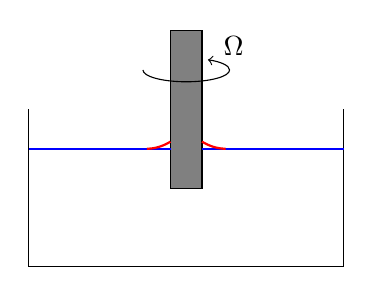
\begin{tikzpicture}
					\draw (-2, 0) -- (2, 0);
					\draw (-2,0) -- (-2, 2);
					\draw (2,0) -- (2, 2);
					\draw[fill=gray] (-0.2,1) rectangle ++ (0.4, 2);
					\draw[blue,thick] (-2, 1.5) -- (-0.2, 1.5);
					\draw[blue,thick] (2, 1.5) -- (0.2,1.5);
					\draw[->] (0, 2.5) [partial ellipse = -180:60:0.55 and
					0.15];
					\draw (0.35, 2.8) node[right] {$\Omega$};
					\draw[red, thick, smooth, samples=100, domain=-0.5:-0.2]
					plot(\x, {1.5+(\x+0.5)^2});
					\draw[red, thick, smooth, samples=100, domain=0.2:0.5]
					plot(\x, {1.5+(\x-0.5)^2});
				\end{tikzpicture}
			\end{center}
			Consider a vertical rod rotating at a constant rate $\Omega$
			placed into a fluid. In a Newtonian fluid, viscous enough for
			Stokes equations to apply, there is no change in the position of
			the interface (blue).

			In a non-Newtonian fluid, the interface climbs up the rod (red).
			This is due to elastic tension: rotation creates circular
			streamlines. Tension along circles creates \emph{hoop stress}
			which `squeezes' the fluid and thus climbs up the rod.

		\item  Particle migration in a pipe flow.
			\begin{center}
				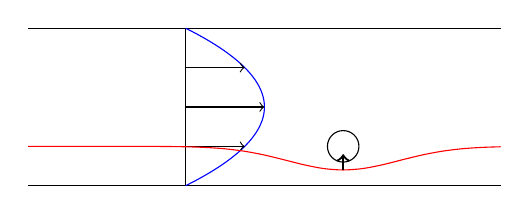
\begin{tikzpicture}
					\draw (-3, 1) -- (3, 1);
					\draw (-3, -1) -- (3, -1);
					\draw (-1, -1) -- (-1, 1);
					\draw[smooth, domain=-1:1, blue, variable=\y] plot ({-\y * \y}, {\y});
					\draw[->] (-1, 0) -- (0, 0);
					\draw[->] (-1, 0.5) -- (-0.25, 0.5);
					\draw[->] (-1, -0.5) -- (-0.25, -0.5);
					\draw (1, -0.5) circle (0.2);
					\draw[smooth,domain=-3:3,red] plot ({\x},
					{-0.5-0.3*exp(-(\x-1)^2)});
					\draw[thick,->] (1,-0.8) -- (1, -0.6);
				\end{tikzpicture}
			\end{center}
			In the case of Newtonian Stokes flow, the flow has no component
			perpendicular to the walls so a particle remains the same distance
			from the wall as it moves along the pipe. In the non-Newtonian
			case, hoop stress caused by curved streamlines lifts the particle
			away from the wall.
	\end{enumerate}
\end{eg}

\subsection{Extensional Viscosity}
A shear flow is a \emph{weak flow}: there is algebraic growth of distances
between particles. In a \emph{strong flow}, distances grow exponentially.

Consider a fluid with extension in the $x$ and $y$ directions and compression
in the $z$ direction: $\bm{u} +
\dot{\varepsilon}\left(\frac{1}{2}x,\frac{1}{2}y, -z\right)$. We call
$\dot{\varepsilon}$ the \emph{extension rate}. Note that this flow is
incompressible. The shear rate tensor is
\begin{equation}
	\dunder{\dot{\gamma}} = \dot{\varepsilon}\begin{pmatrix} 1 & 0 & 0 \\ 0 &
	1 & 0 \\ 0 & 0 & -2 \end{pmatrix}
\end{equation}

In the Newtonian case, the shear rate tensor is
\begin{equation}
	\dunder{\sigma} = \begin{pmatrix}
		-p_0 + \eta \dot{\varepsilon} & 0  & 0 \\
		0 & -p_0 + \eta \dot{\varepsilon} & 0 \\
		0 & 0 & -p_0 -2 \eta \dot{\varepsilon} 
	\end{pmatrix}
\end{equation}

\begin{defn}
	The \emph{extensional viscosity} is
	\begin{equation}
		\eta_{\text{ext}} = \frac{\sigma_{xx}-\sigma_{zz}}{\dot{\varepsilon}}
	\end{equation}
	which has units of viscosity.
\end{defn}

Thus for the Newtonian fluid, $\eta_{\text{ext}} = 3\eta$ which is constant. 
\begin{defn}
	The \emph{Troutou ratio} is 
	\begin{equation}
		\text{Tr} = \frac{\eta_{\text{ext}}}{\eta}
	\end{equation}
\end{defn}

By the above calculations, Newtonian fluids have $\text{Tr} = 3$.
Non-Newtonian fluids tend to have $\text{Tr} \gg 1$ in some range of shear
rates. Thus complex fluids have a very different response to strong flows
compared with weak flows.

\begin{center}
	\begin{tikzpicture}
		\draw[thick,->] (-0.1, 0) -- (5, 0) node[below] {$\dot{\varepsilon}$};
		\draw[thick,->] (0, -0.1) -- (0, 3) node[left] {Tr};
		\draw[dashed] (-0.1, 1) -- (5, 1);
		\draw (-0.1, 1) node[left] {$3$};
		\draw[smooth,blue,domain=0:5] plot({\x},{1+1/(0.5+exp(-2*(\x-3)))});
		\draw (5, 3) node[above] {$\text{Tr} \gg 1$};
	\end{tikzpicture}
\end{center}

\lecture{15/10/20}
\section{Generalised Newtonian Fluids}

We will focus on steady flows and fluids which are \emph{inelastic}. We will
find how to incorporate shear-dependent viscosity into the constitutive
relationship. One way is to generalise the Newtonian constitutive
relationship to
\begin{equation}
	\dunder{\sigma} = -p \dunder{1} +
	\eta(\dunder{\dot{\gamma}})\dunder{\dot{\gamma}}
\end{equation}
where $\eta(\dunder{\dot{\gamma}})$ is found empirically. These are called
\emph{generalised Newtonian fluids} (GNF).

We have a scalar function $\eta$ of a tensor $\dunder{\dot{\gamma}}$, which is
not in general coordinate invariant. Thus $\eta$ must be a function of the
\emph{invariants} of $\dunder{\dot{\gamma}}$. A rank $2$ tensor in $3$
dimensions has $3$ invariants. These are combinations of trace, determinants,
and eigenvalues. We choose as the three invariants:
\begin{equation}
	\trace{\dunder{\srate}}, \hspace{2em} \trace{\dunder{\srate} \cdot
	\dunder{\srate}}, \hspace{2em} \trace{\dunder{\srate} \cdot
\dunder{\srate} \cdot \dunder{\srate}}
\end{equation}

We always have $\trace{\dunder{\srate}} = 0$ because the flow is incompressible:
\begin{equation}
	\trace{\dunder{\srate}} = \dot{\gamma}_{ii} = \frac{\partial u_i}{\partial x_i} +
	\frac{\partial u_i}{\partial x_i} = 2\nabla \cdot \bm{u} = 0
\end{equation}

Consider a simple shear flow $\bm{u} = \dot{\gamma} y \hat{\bm{x}}$. Then
\begin{equation}
	\begin{aligned}
		\dunder{\srate} &= \begin{pmatrix} 0 & \srate & 0 \\ \srate & 0 & 0 \\
		0 & 0 & 0 \end{pmatrix} \\
			\dunder{\srate}\cdot\dunder{\srate} &= \begin{pmatrix} \srate^2 &
			0 & 0 \\ 0 & \srate^2 & 0 \\ 0 & 0 & 0 \end{pmatrix} \\
			\dunder{\srate}\cdot\dunder{\srate}\cdot\dunder{\srate} &=
			\begin{pmatrix} 0 & \srate^3 & 0 \\ \srate^3 & 0 & 0 \\
			0 & 0 & 0 \end{pmatrix}
		\end{aligned}
\end{equation}

Thus $\trace{\dunder{\srate}\cdot\dunder{\srate}\cdot\dunder{\srate}} = 0$ and
$\trace{\dunder{\srate}\cdot\dunder{\srate}} = 2\srate^2$. We assume all flows
are approximately steady shear flow. Then
$\trace{\dunder{\srate}\cdot\dunder{\srate}}$ is the only non-zero invariant
and $\eta(\dunder{\srate}) =
\eta(\trace{\dunder{\srate}\cdot\dunder{\srate}})$.

\begin{defn}
	The \emph{magnitude of shear rate} is
	\begin{equation}
		\srate \equiv
		\left(\frac{\trace{\dunder{\srate}\cdot\dunder{\srate}}}{2}\right)^{1/2}
		= \left(\frac{\dunder{\srate} : \dunder{\srate}}{2}\right)^{1/2}
	\end{equation}
	Note that $\srate \ge 0$ and for a simple shear flow the magnitude of
	shear rate $\srate = \abs{\srate}$ which is the shear rate from steady
	shear flow. Thus the definitions coincide.
\end{defn}

Note the second invariant $\trace{\dunder{\srate}\cdot\dunder{\srate}} =
\dunder{\srate}:\dunder{\srate} \ge 0$ and is zero only when there is no
deformation (since $\dunder{\srate}:\dunder{\srate}$ is proportional to
viscous dissipation), i.e. rigid body motion.

Recall for a simple shear flow, the shear stress is $\sigma =
\eta(\srate)\srate$, thus the above definitions agree with measurements of
shear-dependent viscosity.

\subsection{Power-law fluids}
There are many choices for the function $\eta(\srate)$ for a generalised
Newtonian fluid. Here, we choose a \emph{power-law}
\begin{equation}
	\eta(\srate) \equiv \kappa \srate^{n-1}
\end{equation}
where $\kappa > 0$ and $n \in \ZZ$ is the \emph{power-index} of the fluid.
Note $n=1$ for a Newtonian fluid. For dimensional consistency, we require
$\left[\kappa\right] = \text{Pa}\cdot\text{s}^n$.

\begin{center}
	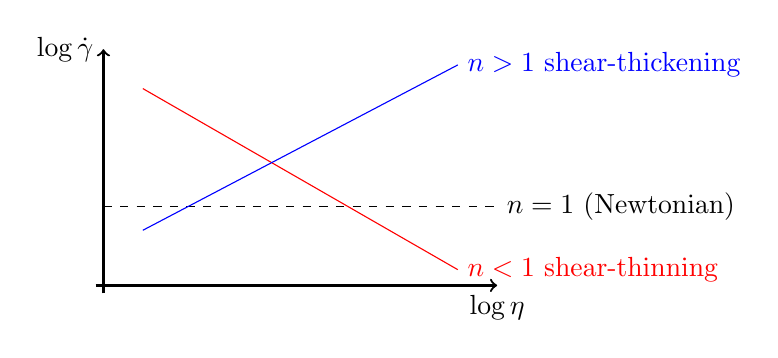
\begin{tikzpicture}
		\draw[thick,->] (-0.1, 0) -- (5, 0) node[below] {$\log \eta$};
		\draw[thick,->] (0, -0.1) -- (0, 3) node[left] {$\log \srate$};
		\draw[dashed] (0,1) -- (5, 1) node[right] {$n=1$ (Newtonian)};
		\draw[red] (0.5, 2.5) -- (4.5, 0.2) node[right] {$n < 1$
		shear-thinning};
		\draw[blue] (0.5, 0.7) -- (4.5, 2.8) node[right] {$n >1$
		shear-thickening};
	\end{tikzpicture}
\end{center}

Note that in the limit $\srate \to 0$, we cannot define a zero-shear rate
viscosity $\eta_0$ unless $n=1$. Thus the model is problematic at small shear
rates. The model is appropriate only for a finite range of shear rates.

\begin{eg}
	Newton's experiment with a power-law fluid. We assume there are no
	external pressures, and the flow is unidirectional: $\bm{u} =
	u(y)\hat{\bm{x}}$. We have
	\begin{equation}
		\dunder{\srate} = \begin{pmatrix} 0 & \frac{\partial u}{\partial y} &
			0 \\ \frac{\partial  u}{\partial y} & 0 & 0 \\ 0 & 0 & 0
		\end{pmatrix}
	\end{equation}

	Then the magnitude of shear rate $\srate = \abs{\frac{\partial u}{\partial
	y}}$. To find the flow, we use the Cauchy equation in 2D:
	\begin{equation}
		\begin{aligned}
			\frac{\partial p}{\partial y} &= 0 \\
			\frac{\partial p}{\partial x} &= \frac{\partial \sigma_{xy}}{\partial y} 
		\end{aligned}
	\end{equation}
	since $\sigma_{xy}$ is the only non-zero component of the shear stress.
	The first equation implies $p = p(x)$ only, which combined with the second
	implies $\sigma_{xy} = \text{const.}$. Note we have not used the
	constitutive relationship yet: this is true for all GNFs. We have
	\begin{equation}
		\sigma_{xy} = \kappa \srate^{n-1} \srate = \kappa \srate^n = \kappa
		\abs{\frac{\partial u}{\partial y}}^n = \text{const.}
	\end{equation}

	Thus $u_y$ is constant, i.e. $u$ is linear in $y$, as with a Newtonian
	fluid. 
\end{eg}

If $\eta(\srate)\srate = \sigma$ is a one-to-one function of $\srate$ then the
result is the same: $u$ varies linearly. A Couette flow $\bm{u} = Uy/h
\hat{\bm{x}}$ is a \emph{viscometric flow}: this flow is realised for all
constitutive relationships provided $\sigma$ is indeed a one-to-one function
of $\srate$.

How do experimentally measure $\eta(\srate)$? One method is a \emph{shear flow
rheometer}:
\begin{enumerate}
	\item Impose $\srate$, measure $\sigma$ (or vice versa)
	\item Measure $\eta = \sigma/\srate$
	\item Repeat varying $\srate$ or $\sigma$
\end{enumerate}

\subsubsection{Pipe flow of a power-law fluid}
\label{sec:pipe}
Consider axisymmetric pressure-driven flow in a pipe of a power-law GNF. If
the fluid was Newtonian, we would get Poiseuille flow with a parabolic flow
profile.

\begin{center}
\begin{tikzpicture}
	\draw (0,0) ellipse (0.6 and 1);
	\draw (0,-1) -- (8,-1);
	\draw (0, 1) -- (8,1);
	\draw (8,0) [partial ellipse = -90:90:0.6 and
	1];
	\draw[dashed] (8,0) [partial ellipse = 90:270:0.6 and
	1];
	\draw[thick,blue,->] (4,0) -- (6, 0) node[right] {flow};
	\draw (-2, 0) node {$p_0 + \Delta p$};
	\draw (10, 0) node {$p_0$};
	\draw[->] (0,0) -- (0,1) node[midway,right] {$R$};
	\draw[<->] (0,-1.5) -- (8,-1.5) node[midway, below] {$L$};
\end{tikzpicture}
\end{center}

We will use cylindrical coordinates $(r,\theta,z)$ and assume the flow is
unidirectional: $\bm{u} = u(r)\hat{\bm{z}}$. Then
\begin{equation}
	\dunder{\srate} = \begin{pmatrix} 0 & 0 & \frac{\partial u}{\partial r} \\
	0 & 0 & 0 \\ \frac{\partial u}{\partial r} & 0 & 0 \end{pmatrix}
\end{equation}

The magnitude of shear rate $\srate = \abs{\frac{\partial u}{\partial r}}$.
The Cauchy equations in cylindrical coordinates are
\begin{equation}
	\begin{aligned}
		\frac{\partial p}{\partial r} &= 0 \\
		\frac{\partial p}{\partial \theta} &= 0 \\
		\frac{\partial p}{\partial z} &= \frac{1}{r} \frac{\partial}{\partial
		r} \left( r \sigma_{rz}\right)
	\end{aligned}
\end{equation}

since $\sigma_{rz}$ is the only non-zero component of shear stress. The first
two equations imply $p = p(z)$. Then $\frac{\partial p}{\partial z}$ is a
function of $z$ only, but the RHS is a function of $r$ only. Thus each
must be constant. Then
\begin{equation}
	\frac{\partial p}{\partial z} = -\frac{\Delta p}{L} \implies \sigma_{rz} =
	-\frac{\Delta p}{2L} r + \frac{A}{r}
\end{equation}

The $A/r$ term is singular at $r=0$ thus $A \equiv 0$. Note these results are
true for all guids - we have not yet used the fact this is a power-law fluid.

Denote the \emph{magnitude of wall shear stress} as $\sigma_w$. In this case,
$\sigma_w = \frac{\Delta p}{2L}R$.  To find the flow field, we need the
constitutive relationship. For a GNF we have
\begin{equation}
	\sigma_{rz} = \eta\left(\abs{\frac{\partial u}{\partial r}}\right)
	\frac{\partial u}{\partial r} = -\frac{\Delta p}{2L} r
\end{equation}

We expect $u$ to be at maximum when $r=0$, so expect $\frac{\partial
u}{\partial r} < 0$. Thus $\abs{u_r} = -u_r$. For a power-law fluid, $\sigma =
\kappa \srate^n$, thus
\begin{equation}
	\begin{aligned}
		\kappa \abs{\frac{\partial u}{\partial r}}^n &= \frac{\Delta p}{2L} r
		\\
		\implies \abs{\frac{\partial u}{\partial r}} &= \left(\frac{\Delta p}{2
		L \kappa}\right)^{1/n} r^{1/n} = -\frac{\partial u}{\partial r} \\
		\implies u(r) &= C - \left(\frac{\Delta p}{2 L \kappa}\right)^{1/n}
		\frac{n}{n+1} r^{\frac{n+1}{n}}
	\end{aligned}
\end{equation}

Enforcing no-slip boundary conditions on the pipe wall $u(R) = 0$ and
re-writing in terms of the wall shear stress we have
\begin{equation}
	u(r) = \left(\frac{\sigma_w}{\kappa R}\right)^{1/n} \frac{n}{n+1}\left(
	R^{\frac{n+1}{n}} - r^{\frac{n+1}{n}}\right)
\end{equation}

We can calculate the mean flow speed $\bar{U}$:
\begin{equation}
	\bar{U} \equiv \frac{1}{\pi R^2} \iint u \, \diffd S = \frac{2}{R^2}
	\int_0^R ru(r) \, \diffd r = \left(\frac{\sigma_w}{\kappa}\right)^{1/n}
	\frac{nR}{3n+1}
\end{equation}

Finally, we can rewrite the solution as flow relative to the mean flow speed:
\begin{equation}
	\frac{u(r)}{\bar{U}} = \frac{3n+1}{n+1} \left[ 1-
	\left(\frac{r}{R}\right)^{\frac{n+1}{n}}\right]
\end{equation}

\begin{center}
	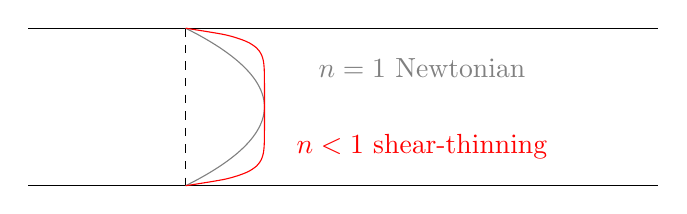
\begin{tikzpicture}
		\draw (0, 1) -- (8, 1);
		\draw (0, -1) -- (8, -1);
		\draw[dashed] (2,1) -- (2,-1);
		\draw[smooth,gray,domain=-1:1,variable=\y] plot ({3-\y*\y},{\y});
		\draw[smooth,red,domain=-1:1,variable=\y] plot
		({3-\y*\y*\y*\y*\y*\y*\y*\y},{\y});
		\draw[gray] (5, 0.5) node {$n=1$ Newtonian};
		\draw[red] (5, -0.5) node {$n < 1$ shear-thinning};
	\end{tikzpicture}
\end{center}

Physically, we have high shear near the pipe walls, so low viscosity in a
shear-thinning complex fluid. The flow rate is
\begin{equation}
	Q = \iint u \, \diffd S = \frac{\pi n}{3n+1} \left(\frac{\Delta p}{2 L
	\kappa}\right)^{1/n} R^{3+\frac{1}{n}}
\end{equation}

For a Newtonian fluid, $Q \sim \Delta p R^4$ whereas for a power-law fluid $Q
\sim \Delta p ^{1/n} R^{3+\frac{1}{n}}$. For a shear-thinning fluid with $n <
1$, we thus have a very strong dependence on $\Delta p$ and $R$. In a device
with $Q$ fixed, $\Delta p^{1/n} R^{3+\frac{1}{n}} = \text{const.}$ so $\Delta
p \sim R^{-(3n+1)}$. For $n < 1$, it is therefore easier to push fluid through
a pipe than with a Newtonian fluid.

\lecture{20/10/20}
\subsection{Other models \& problems}
\subsubsection{Carreau-Yasuda model}
The Carreau-Yasuda model can be written
\begin{equation}
	\frac{\eta(\srate)-\eta_\infty}{\eta_0 - \eta_\infty} = \left[ 1 +
	(\lambda \srate)^a\right]^{n-1}{a}
\end{equation}
for $n \le 1$. In this model, $\eta$ transitions smoothly from $\eta_0$ to
$\eta_\infty$. In some finite range of shear rates, the model resembles a
power-law fluid. In fact, a power-law fluid can be thought of as a `subset' of
Carreau-Yasuda. The constant parameter $a$ is related to the curvature of the
$\eta$ vs. $\srate$ curve, whilst $n$ is related to the steepness of the
curve.

\begin{center}
	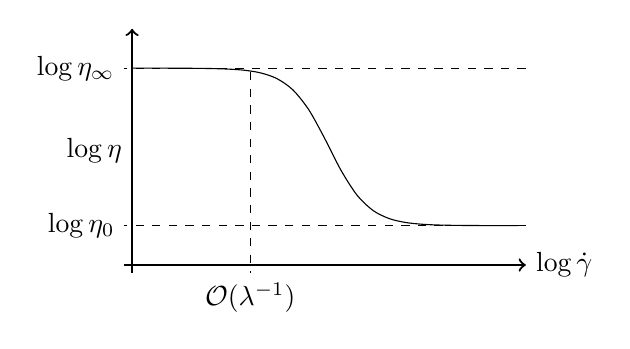
\begin{tikzpicture}
		\draw[thick,->] (-0.1, 0) -- (5,0) node[right] {$\log \srate$};
		\draw[thick,->] (0,-0.1) -- (0, 3) node[left,midway] {$\log \eta$};
		\draw[smooth,domain=0:4.9] plot({\x},{2/(1+exp(4*\x-10))+0.5});		
		\draw[dashed] (5,0.5) -- (-0.1,0.5) node[left] {$\log \eta_0$};
		\draw[dashed] (5,2.5) -- (-0.1, 2.5) node[left] {$\log \eta_\infty$};
		\draw[dashed] (1.5,2.45) -- (1.5,-0.1) node[below] {$\mathcal{O}(\lambda^{-1})$};
	\end{tikzpicture}
\end{center}

\subsubsection{Powell-Eyring \& Ellis models}
The Powell-Eyring model is given by
\begin{equation}
	\frac{\eta(\srate)-\eta_\infty}{\eta_0 - \eta_\infty} =
	\frac{\sinh^{-1}(\lambda \srate)}{\lambda \srate}
\end{equation}

Some models specify $\eta(\sigma)$ instead of $\eta(\srate)$, for example the
Ellis model.
\begin{equation}
	\eta = \eta_0 \left[ 1 + \abs{\frac{\sigma}{\sigma_0}}^{1-n}\right]^{-1}
\end{equation}

There are several properties and issues associated with generalised Newtonian
fluids.
\begin{enumerate}
	\item Empirical: GNFs are based on experiments rather than derived.
	\item Instantaneous: GNFs have no memory (recall the step shear
		experiment), so are not suitable for modelling unsteady flows. This
		also means GNFs are instantaneously reversible which is undesired.
	\item No normal stress differences.
	\item Under extension, the Troutou ratio is $\text{Tr} = 3$ for GNFs, i.e.
		there is no increase in extensional viscosity.

	\item The behaviour of stress when $\srate \to 0$ is important. If
		$\eta_0$ can be defined, then $\sigma \to 0$. If not, such as with a
		power-law fluid, there is problematic behavoiur near $0$. The limit
		$\srate \to 0$ is often used to recover Newtonian behaviour.
\end{enumerate}

\subsection{Rheometry}
\emph{Rheometry} is the science and engineering of measuring material
properties of fluids. For generalised Newtonian fluids, we need to measure
$\eta(\srate)$. The `easy' method is to use a steady shear flow, which is
simple in principle. However, we can only use a finite volume of fluid. A
common solution is the \emph{parallel plate rheometer}, also known as a
parallel disc rheometer. 

Consider two coaxial rigid circular discs of radius $a$ held at a constant separation
$h$. The bottom plate is held stationary whilst the upper plate rotates at a
prescribed angular velocity $\Omega$. The variable $\srate$ is controlled in
this experiment.

\begin{center}
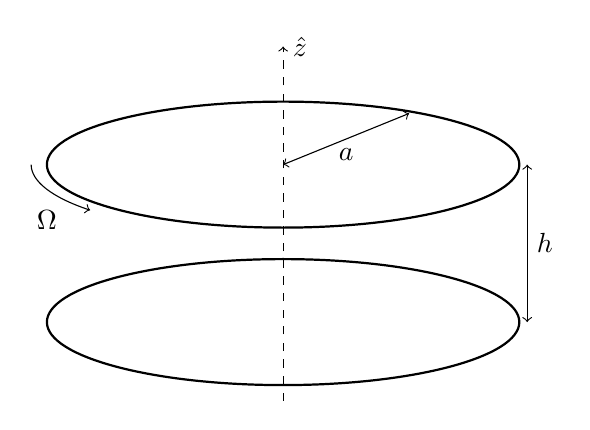
\begin{tikzpicture}
	\draw[thick] (0,0) ellipse (3 and 0.8);
	\draw[thick] (0,-2) ellipse (3 and 0.8);
	\draw[dashed, ->] (0,-3) -- (0,1.5) node[right] {$\hat{\bm{z}}$};
	\draw[<->] (0,0) -- (1.6,0.65) node[midway,below] {$a$};
	\draw[<->] (3.1, 0) -- (3.1, -2) node[midway,right] {$h$};
	\draw[->] (0, 0) [partial ellipse = -180:-140:3.2 and
	0.9];
	\draw (-3, -0.7) node {$\Omega$};
\end{tikzpicture}
\end{center}

The input-output relationship can be inverted to infer $\eta(\srate)$. Use
cylindrical coordinates $(r, \theta, z)$ and look for an axisymmetric flow
field $\bm{u} = u(r,z) \hat{\bm{\theta}}$. The shear rate tensor is
\begin{equation}
	\dunder{\srate} = \begin{pmatrix} 0 & r\frac{\partial}{\partial r} \left(
		\frac{u}{r}\right) & 0 \\ r\frac{\partial}{\partial r} \left(
	\frac{u}{r}\right) & 0 & \frac{\partial u}{\partial z} \\
0 & \frac{\partial u}{\partial z} & 0 \end{pmatrix}
\end{equation}

Consider the steady Cauchy equation in cylindrical coordinates:
\begin{align}
	\frac{\partial p}{\partial \theta} &= 0 = \frac{1}{r^2} \frac{\partial
		}{\partial r} \left( r^2 \tau_{r\theta}\right) + \frac{\partial}{\partial
z}\left( \tau_{\theta z}\right) \\
\frac{\partial p}{\partial r} &= 0 \\ \frac{\partial p}{\partial z} &= 0
\end{align}


We wish to find a viscometric flow solution. In the Newtonian case, we have
\begin{equation}
	0 = \frac{1}{r^2} \frac{\partial
		}{\partial r} \left( r^3 \frac{\partial}{\partial r} \left(
	\frac{u}{r}\right)\right) + \frac{\partial^2 u}{\partial z^2}\\
\end{equation}

To find a solution we require both terms vanish. Thus $u = A(r) z + B(r)$. The
no-slip boundary condition $u = 0$ at $z=0$ and $u = \Omega r$ at $z = h$
gives
\begin{equation}
	u(r,z) = \Omega r \frac{z}{h}
\end{equation}

Given this flow, the shear rate tensor becomes
\begin{equation}
	\dunder{\srate} = \begin{pmatrix} 0 & 0 & 0 \\ 
		0 & 0 & \frac{r \Omega}{h} \\
0 & \frac{r \Omega}{h} & 0 \end{pmatrix}
\end{equation}

Assume $\Omega > 0$, so the magnitude of the shear rate is $\srate =
\abs{r\Omega/h}$. This solution is also a solution for a GNF: we have
$\tau_{r\theta} = 0$ and 
\begin{equation}
	\tau_{\theta z} = \eta(\srate) \srate =
	\eta(\frac{r\Omega}{h})\frac{r\Omega}{h} = \tau_{\theta z} (r)
\end{equation}

The torque exerted to rotate the top plate is $\bm{T} = T\hat{\bm{z}}$ where
\begin{equation}
	T = \int r \tau_{\theta z} \, \diffd S = 2\pi \int_0^a r^2 \eta(\srate)
	\srate \, \diffd r
\end{equation}

This relationship can be used to infer $\eta(\srate)$ by a change of variable.
Let $\srate_a = a\Omega/h$ be the shear rate at the edge of the disc.
Substitute $r = a \srate/\srate_a$:
\begin{equation}
	T = 2\pi \int_0^{\srate_a} \frac{a^2}{\srate_a^2} \srate^2
	\eta(\srate)\srate \frac{a}{\srate_a} \, \diffd \srate = 2\pi
	\frac{a^3}{\srate_a^3} \int_0^{\srate_a} \eta(\srate) \srate^3 \, \diffd
	\srate
\end{equation}
This is valid for all values of $\srate_a$. Rearranging and differentiating
with respect to $\srate_a$ we have
\begin{equation}
	\eta(\srate_a) = \frac{1}{\srate_a^3} \frac{\diffd}{\diffd \srate^a}
	\left[ \frac{T \srate_a^3}{2\pi a^3}\right]
\end{equation}

In an experiment, we control $\srate_a$, measure $T$, slightly change
$\srate_a$, and repeat. Application of the above result then yields
$\eta(\srate_a)$. Other geometries can also be used:
\begin{itemize}
	\item Taylor-Couette.
		\begin{center}
			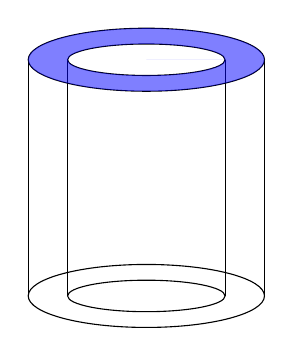
\begin{tikzpicture}
				\draw[name path =A] (0,0) ellipse (1 and 0.2);
				\draw[name path =B] (0,0) ellipse (1.5 and 0.4);
				\draw (0,-3) ellipse (1 and 0.2);
				\draw (0,-3) ellipse (1.5 and 0.4);
				\draw (1.5,0) -- (1.5, -3);
				\draw (-1.5, 0) -- (-1.5, -3);
				\draw (1, 0) -- (1, -3);
				\draw (-1, 0) -- (-1, -3);
				\tikzfillbetween[of=A and B]{blue, opacity=0.5}
			\end{tikzpicture}
		\end{center}
	\item Cone and plate. Useful since $\alpha$ small implies the shear rate
		$\srate$ is uniform.
		\begin{center}
			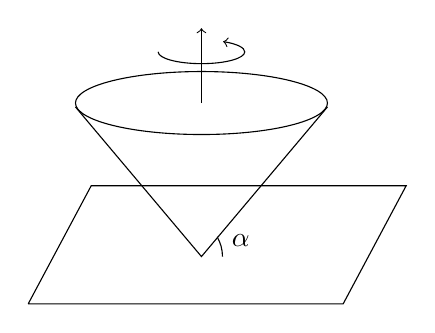
\begin{tikzpicture}
				\draw (-2,0) -- (2,0) -- (2.8, 1.5) -- (-1.2, 1.5) -- (-2,0);
				\draw (-1.4, 2.5) -- (0.2, 0.6) -- (1.8, 2.5);
				\draw (0.2, 2.55) ellipse (1.6 and 0.4);
				\draw (0.4, 0.85) arc (30:0:0.5);
				\draw (0.7, 0.8) node {$\alpha$};
				\draw[->] (0.2, 2.55) -- (0.2, 3.5);
				\draw[->] (0.2, 3.2) [partial ellipse = -180:60:0.55 and
				0.15];
			\end{tikzpicture}
		\end{center}
\end{itemize}

\lecture{22/10/20}
\subsection{Variational approach}
So far, we have found exact solutions only. For many GNF, no exact solutions
are available so we must find approximate solutions. Here we consider a method
relying on a form of energy minimisation. Conider a fluid volume V, bounded by
a surface S, in the Stokes flow limit (no inertia). Assume $\bm{u} = \bm{u}_0$
is prescribed on $S$. The total rate of energy dissipation is
\begin{equation}
	P = \int_V \frac{1}{2}\dunder{\sigma}:\dunder{\srate}\,\diffd V = \int_V
	\frac{\eta}{2} \dunder{\srate}:\dunder{\srate} \, \diffd V \ge 0
\end{equation}

Recall the minimum dissipation theorem: solutions to Stokes equations minimise
$P$ over all incompressible flows satisfying the same boundary conditions. The
inequality $P_{\text{Stokes}} \le P$ can be shown directly, or we can use the
calculus of variations. Define a Lagrangian
\begin{equation}
	\mathcal{L} \equiv P + \int_V \lambda \nabla \cdot \bm{u} \, \diffd V
\end{equation}

Variations with respect to $\lambda$ give $\nabla \cdot \bm{u} = 0$, and
variations with respect to $\bm{u}$ give Stokes equations with pressure $p
\propto \lambda$. To generalise this to GNF, consider the power density $f =
\frac{1}{2}\eta \srate^2$ for a Newtonian fluid. Analogously, for a GNF we define
\begin{equation}
	f = \int_0^{\srate} \eta(x)x\, \diffd x
\end{equation}
and a new Lagrangian
\begin{equation}
	\mathcal{L} \equiv \mathcal{L}\left[\bm{u},\lambda\right] = \int_V f \, \diffd
	V + \int_V \lambda \nabla \cdot \bm{u}\,\diffd V
\end{equation}

\subsubsection{Calculus of variations}
Consider a functional $J$ of a vector field $\bm{y}(\bm{x})$ and its
spatial derivatives $y_{m,n} \equiv \frac{\partial y_m}{\partial x_n}$;
\begin{equation}
	J\left[\bm{y}\right] = \int_V F(x_i,y_j,y_{m,n}) \, \diffd V
\end{equation}
where $V$ is the total domain. The \emph{first variation} of $J$ is $\delta J$ where
\begin{equation}
	J + \delta J = J\left[\bm{y}+\delta\bm{y}\right] = \int_V
	F(\bm{x},\bm{y}+\delta\bm{y})\,\diffd V
\end{equation}
To determine an explicit expression for the first variation, first Taylor
expand the integrand:
\begin{equation}
	F(\bm{x},\bm{y}+\delta\bm{y}) = F + \delta y_j \frac{\partial F}{\partial
		y_j} + \delta y_{m,n} \frac{\partial F}{\partial y_{m,n}} + \dots
\end{equation}
Using integration by parts and writing $\delta y_{m,n} =
\frac{\partial}{\partial x_n} \delta y_m$ we have
\begin{equation}
	\delta y_{m,n} \frac{\partial F}{\partial y_{m,n}} = 
	\frac{\partial}{\partial x_n}\left( \delta y_m \frac{\partial F}{\partial
		y_{m,n}}\right) - \delta y_m \frac{\partial}{\partial x_n} \left(
	\frac{\partial F}{\partial y_{m,n}}\right)
\end{equation}

The first term becomes a surface integral via Stokes' theorem, which may or
may not vanish depending on boundary conditions. The first variation of $F$ is
thus
\begin{equation}
	\delta F = \delta y_j \left[ \frac{\partial F}{\partial y_j} -
		\frac{\partial}{\partial x_n} \left( \frac{\partial F}{\partial
	y_{j,n}}\right)\right] + \text{boundary terms}
\end{equation}

Now requiring $\delta J = 0$ for all $\delta y$ is equivalent to requiring
$\delta F = 0$ for all $\delta y$, giving the \emph{Euler-Lagrange equation}.
\begin{equation}
\frac{\partial F}{\partial y_j} - \frac{\partial}{\partial x_n} \left(
\frac{\partial F}{\partial y_{j,n}}\right) = 0
\end{equation}

\subsubsection{Variational solution}
Returning to our original set-up, denote $F_2 = \lambda \nabla \cdot \bm{u}$,
$F_1 = \int_0^{\srate} \eta(x)x\,\diffd x$, so
\begin{equation}
	\mathcal{L}\left[\bm{u},\lambda\right] = \int_V F_1 + F_2\,\diffd V
\end{equation}

Note that we are using $\bm{y} \equiv \bm{u}$ here.  The Euler-Lagrange
equation for $\lambda $ gives
\begin{equation}
	\frac{\partial}{\partial \lambda} \left( F_1 + F_2\right) = 0 \implies
	\nabla \cdot \bm{u} = 0
\end{equation}

For variations with respect to $\bm{u}$, we have boundary terms involving
$\delta \bm{u}$. Since $\delta \bm{u} = \bm{0}$ on $S$, the boundary terms
vanish in this case. There is no explicit dependence on $\bm{u}$ in $F_1, F_2$
so the Euler-Lagrange equation becomes
\begin{equation}
	\frac{\partial}{\partial x_n} \left( \frac{\partial F}{\partial
	u_{j,n}}\right) = 0
\end{equation}

where $F \equiv F_1 + F_2$. By chain rule, 
\begin{equation}
	\frac{\partial F_1}{\partial u_{j,n}} = \frac{\partial \srate}{\partial
	u_{j,n}} \frac{\partial F_1}{\partial \srate}
\end{equation}
We have $\frac{\partial F_1}{\partial \srate} = \eta(\srate) \srate$ and
\begin{align}
	\frac{\partial \srate}{\partial u_{j,n}} &=
	\frac{1}{2\srate} \frac{\partial}{\partial u_{j,n}} \left( \frac{1}{2}
	\dunder{\srate}:\dunder{\srate}\right) \\
	&= \frac{1}{2\srate} \frac{\partial}{\partial u_{j,n}} \left( \frac{1}{2}
	\srate_{pq} \srate_{pq}\right) \\
	&= \frac{1}{4\srate} \frac{\partial}{\partial u_{j,n}}\left(
u_{p,q}u_{p,q} + 2u_{p,q}u_{q,p} + u_{q,p}u_{q,p}\right) \\
&= \frac{1}{2\srate} \left( 2 u_{j,n} + 2u_{n,j}\right) \\
&= \frac{\srate_{jn}}{\srate}
\end{align}

Now for $F_2 = \lambda \nabla \cdot \bm{u}$ we have
\begin{align}
	\frac{\partial}{\partial x_n} \left( \frac{\partial F_2}{\partial u_{j,n}}
		\right) &= \frac{\partial}{\partial x_n} \left( \lambda
		\frac{\partial u_{i,i}}{\partial u_{j,n}}
	\right) \\
	&= \frac{\partial}{\partial x_n} \left( \lambda \delta_{ij}
\delta_{in}\right) \\
&= \frac{\partial \lambda}{\partial x_j}
\end{align}

Thus the full Euler-Lagrange equation for $\bm{u}$ is
\begin{equation}
	\frac{\partial}{\partial x_n} \left[ \eta(\srate) \srate_{jn}\right] +
	\frac{\partial \lambda}{\partial x_j} = 0
\end{equation}
for $j= 1, 2, 3$. Given $\lambda = -p$, this becomes the Cauchy equation for a
GNF.
\begin{equation}
	-\nabla p + \nabla \cdot \left[ \eta(\srate) \dunder{\srate}\right] =
	\bm{0}
\end{equation}

Pressure is used as a Lagrange multiplier to enforce incompressibility. Note:
if the boundary conditions are different, e.g. $\dunder{\sigma} \cdot \bm{n}$
is prescribed, we must distinguish surfaces where $\bm{u}$ is described and
surfaces where $\dunder{\sigma} \cdot \bm{n}$ is prescribed, and add a surface
integral to the Lagrangian (see Example Sheet 1).

To generate approximate solutions to the Cauchy GNF equations, we note that
the closer the value of $\mathcal{L}$ to its minimum, the better the
approximation. Thus
\begin{enumerate}
	\item Use incompressible test functions $\bm{u}_\alpha$ where $\alpha$ is
		a parameter
	\item Substitute into Lagrangian, minimise with respect to $\alpha$
	\item If the minimum of $\mathcal{L}$ is at $\alpha = \alpha^*$ then
		$\bm{u}_{\alpha^*}$ is an approximate solution
\end{enumerate}

Integrals involved in $\mathcal{L}$ in general have to be evaluated
numerically. Choice of test functions comes from physical intuition,
computation, or experiment.

\lecture{27/10/20}
\section{Yield-Stress Fluids}
Some fluids only flow when subject to stress above some threshold. We call
this threshold the \emph{yield-stress}, denoted by $\sigma_y$. Fluids with such
a property are called \emph{yield-stress fluids} or \emph{viscoplastic fluids}.
Examples are mayonnaise; jelly; peanut butter; mud; and hair gel. Graphically,
$\sigma_y$ is the non-zero $\srate$-intercept of $\sigma(\srate)$. Beyond the
yield-stress, the fluid may have Newtonian, shear-thinning, shear-thickening,
or some other behaviour. 

The simplest model of a yield-stress fluid is a \emph{Bingham fluid} where the
behaviour is Newtonian beyond the yield-stress. For $-\infty < \srate <
\infty$ we have
\begin{equation}
	\begin{cases}
		\srate = 0 & \abs{\sigma} < \sigma_y \\
		\sigma = \text{sgn}(\srate)\sigma_y + \eta \srate & \abs{\sigma} > \sigma_y
	\end{cases}
\end{equation}

Alternatively, non-linear behaviour after yield is described by the
\emph{Herschel-Bulkley model} where the fluid has power-law behaviour after
yield. 
\begin{equation}
	\begin{cases}
		\srate = 0 & \abs{\sigma} < \sigma_y \\
		\sigma = \text{sgn}(\srate)\sigma_y + \kappa \abs{\srate}^{n-1} \srate
		& \abs{\sigma} > \sigma_y 
	\end{cases}
\end{equation}

\begin{center}
	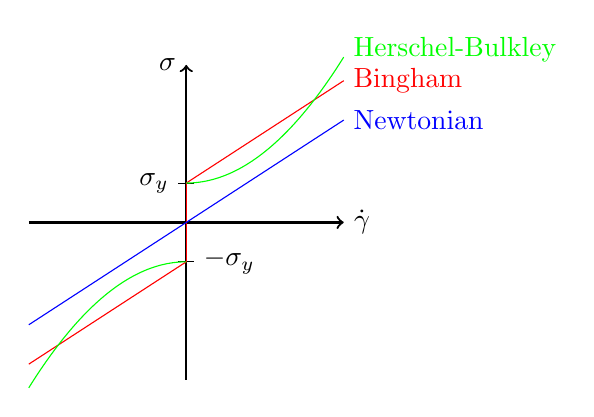
\begin{tikzpicture}
		\draw[thick,->] (-2, 0) -- (2,0) node[right] {$\srate$};
		\draw[thick,->] (0,-2) -- (0, 2) node[left] {$\sigma$};
		\draw (0.1, 0.5) -- (-0.1, 0.5) node[left] {$\sigma_y$};
		\draw (-0.1, -0.5) -- (0.1, -0.5) node[right] {$-\sigma_y$};
		\draw[red] (0, -0.5) -- (0, 0.5);
		\draw[red] (0, 0.5) -- (2, 1.8) node[right] {Bingham};
		\draw[red] (0, -0.5) -- (-2, -1.8);
		\draw[blue] (-2,-1.3) -- (2,1.3) node[right] {Newtonian};
		\draw[green, smooth] plot[domain=0:2] ({\x},{0.5+0.4*\x*\x});
		\draw[green, smooth] plot[domain=-2:0] ({\x},{-0.5-0.4*\x*\x});
		\draw[green] (2,2.2) node[right] {Herschel-Bulkley};
	\end{tikzpicture}
\end{center}

A typical flow problem of yield-stress fluids separates the domain into two
regions.
\begin{enumerate}
	\item Yielded domain: the fluid flows in regions where $\abs{\sigma} >
		\sigma_y$
	\item Unyielded domain: where $\abs{\sigma} < \sigma_y$, there is no
		deformation i.e. rigid body motion only
\end{enumerate}

The surface separating the yielded and unyielded regions is the \emph{yield
surface}. On this surface, $\sigma = \sigma_y$ by definition, which implicitly
defines the surface. Physically, we expect high shear at boundaries, and thus
expect the yield surface is close to these boundaries.

\subsection{Pressure-driven flow of a Bingham fluid in a pipe}
This problem illustrates a steady flow problem and the location of the yield
surface. We will use cylindrical coordinates, and assume the flow is
unidirectional with $\bm{u} = u(r) \hat{\bm{z}}$.

\begin{center}
\begin{tikzpicture}
	\draw (0,0) ellipse (0.6 and 1);
	\draw (0,-1) -- (8,-1);
	\draw (0, 1) -- (8,1);
	\draw (8,0) [partial ellipse = -90:90:0.6 and
	1];
	\draw[dashed] (8,0) [partial ellipse = 90:270:0.6 and
	1];
	\draw[thick,blue,->] (4,0) -- (6, 0) node[right] {flow};
	\draw (-2, 0) node {$p_0 + \Delta p$};
	\draw (10, 0) node {$p_0$};
	\draw[->] (0,0) -- (0,1) node[midway,right] {$R$};
	\draw[<->] (0,-1.5) -- (8,-1.5) node[midway, below] {$L$};
\end{tikzpicture}
\end{center}

The Cauchy equation in cylindrical polars (as seen in section~\ref{sec:pipe})
gives
\begin{equation}
	\frac{\partial p}{\partial z} = \frac{1}{r} \frac{\partial}{\partial r}
	\left( r \sigma_{rz} \right) = -\frac{\Delta p}{L}
\end{equation}
thus as before we find
\begin{equation}
	\sigma_{rz} = -\frac{\Delta p}{2L} r
\end{equation}
We wish to find the yield surface. Clearly near $r=0$ the stress is small
so the fluid is unyielded. The yield surface is defined by $\abs{\sigma} =
\sigma_y$ thus we have
\begin{equation}
	r = r_y = \frac{2L}{\Delta p} \sigma_y
\end{equation}
Recall $R$ is the radius of the pipe. Comparing $R$ with $r_y$,
\begin{enumerate}
	\item if $r_y \ge R$ the shear stress is below yield stress thoughout the
		pipe, thus there is no flow. Equivalently, this occurs for pressure
		differences $\Delta p \le \frac{2L}{R} \sigma_y$.
	\item if $r_y < R$ (equivalently $\Delta p > \frac{2L}{R} \sigma_y$) the
		fluid yields in $r_y \le r \le R$, and is unyielded in $0 \le r \le
		r_y$.
\end{enumerate}

We solve case 2 exactly. Flow in the yielded region has $\srate =
\frac{\partial u}{\partial r} < 0$. For a Bingham fluid $\sigma =
\text{sgn}(\srate) \sigma_y + \eta \srate$. Therefore we have
\begin{equation}
	\sigma_{rz} = -\sigma_y + \eta \frac{\partial u}{\partial r}
\end{equation}
Now $\sigma_{rz} = -\frac{\Delta p}{2L} r$ can be rewritten in terms of the
yield surface as $\sigma_{rz} = -\sigma_y \frac{r}{r_y}$. Thus we must solve
\begin{equation}
	\frac{\partial u}{\partial r} = \frac{\sigma_y}{\eta}\left( 1 -
	\frac{r}{r_y}\right)
\end{equation}
Note $r = r_y$ implies $\frac{\partial u}{\partial r} = 0$ which gives
$\abs{\sigma} = \sigma_y$ as expected. We have
\begin{equation}
u(r) = \frac{\sigma_y}{\eta} \left(r - \frac{r^2}{2r_y}\right) + c
\end{equation}
The constant of integration is determined by the no-slip boundary condition on
$r=R$, $u(R) = 0$. Finally we have for $r_y \le r \le R$
\begin{equation}
	u(r) = \frac{\sigma_y}{\eta} \left( r - \frac{r^2}{2r_y} - R +
	\frac{R^2}{2r_y}\right)
\end{equation}

In the unyielded region we have plug flow $u =$ constant.  For $0 \le r \le
r_y$, the rigid body velocity $u = U_y = u_{\text{yielded}}(r_y)$ by
continuity.
\begin{equation}
	\implies U_y = \frac{\sigma_y}{\eta} \left( \frac{r_y}{2} - R +
	\frac{R^2}{2r_y}\right) \ge 0
\end{equation}

The flow profile in the pipe is a combination of parabolic and constant
velocity.
\begin{center}
	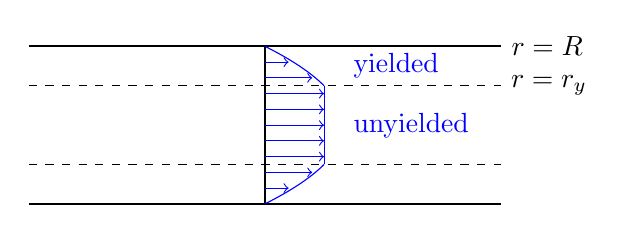
\begin{tikzpicture}
		\draw[thick] (-3, 1) -- (3, 1) node[right] {$r=R$};
		\draw[thick] (-3, -1) -- (3, -1);
		\draw (0, 1) -- (0, -1);
		\draw[dashed] (-3, 0.5) -- (3, 0.5) node[right] {$r=r_y$};
		\draw[dashed] (-3, -0.5) -- (3, -0.5);
		\draw[smooth,blue,domain=-1:-0.5,variable=\y] plot({1-\y*\y},{\y});
		\draw[smooth,blue,domain=1:0.5,variable=\y] plot({1-\y*\y},{\y});
		\draw[blue] (0.75, 0.5) -- (0.75, -0.5);
		\draw (1, 0) node[blue,right] {unyielded};
		\draw (1, 0.75) node[blue,right] {yielded};
		\draw[blue,->] (0,0.4) -- (0.75, 0.4);
		\draw[blue,->] (0,0.2) -- (0.75, 0.2);
		\draw[blue,->] (0,0) -- (0.75,0);
		\draw[blue,->] (0,-0.4) -- (0.75, -0.4);
		\draw[blue,->] (0,-0.2) -- (0.75, -0.2);
		\draw[blue,->] (0,0.6) -- (0.6, 0.6);
		\draw[blue,->] (0,0.8) -- (0.3, 0.8);
		\draw[blue,->] (0,-0.6) -- (0.6, -0.6);
		\draw[blue,->] (0,-0.8) -- (0.3, -0.8);
	\end{tikzpicture}
\end{center}

The flow rate $Q$ vanishes if $r_y \ge R$. For $r_y < R$, 
\begin{align}
	Q &= 2\pi \int_0^R r u(r) \, \diffd r \\
	  &= 2\pi \int_0^{r_y} rU_y \, \diffd r + 2\pi \int_{r_y}^R ru(r) \,
	\diffd r \\
	&= \dots \\
	&= \frac{\Delta p \pi R^4}{8\mu L} \left[ 1 - \frac{4}{3}\frac{r_y}{R} +
	\frac{1}{3} \left( \frac{r_y}{R}\right)^3\right]
\end{align}

The constant factor outside the brackets is the \emph{Hagen-Poiseuille flow
rate} for a Newtonian fluid.
\begin{itemize}
	\item If $r_y = 0$ the fluid is yielded everywhere and we have the
		Newtonian solution for Poiseuille flow in a pipe.
	\item If $r_y = R$ the fluid is unyielded everywhere and $Q = 0$.
	\item The term in brackets is always smaller than $1$, thus
		$Q_{\text{yield-stress}} \le Q_{\text{Newtonian}}$
\end{itemize}

This problem is doable because it is a steady problem. It is much more
difficult in the unsteady case since the yield surface has unsteady motion, in
which case inertia is needed.

\end{document}
